\chapter{Versuch}
In dem Versuch soll getestet werden, ob der Nutzen von Trackern die Performanz und das Embodiment eines Nutzers gegenüber einer Inverse-Kinematik Lösung für selbst Avatare erhöht. Es wurden zwei Gruppen getestet, die miteinander verglichen werden. Eine Gruppe durchläuft das Experiment mit einem durch IK animierten Avatar. Der Avatar der anderen Gruppe wird mithilfe von sechs zusätzlichen Trackern durch die Bewegungen der Testperson animiert.


\section{Konzeption}
Alle Entscheidungen im Versuchsaufbau basieren darauf, den Fokus auf die Animation des Avatars zu legen. Alles andere, was zu unterschiedlichen Reaktionen hinsichtlich des Embodiments führen könnte, wurde weggelassen. So befindet man sich in einem abstrakten, größtenteils leeren Raum. Die einzige eingesetzte Textur ist die auf dem Boden, da so in den Tests die Entfernung zu den Objekten besser bestimmt werden konnte. Vor allem die bewusste Entscheidung, dem Avatar keine Kleidung zu geben und ihn als Holzpuppe darzustellen. Verschiedene Personen könnten sich mit der Kleidung mehr oder weniger Identifizieren und so könnte der Fokus von den Animationen abgelenkt werden, vor allem da der Avatar eine Zentrale Rolle im Versuch spielt.
Es wird kein Ton eingesetzt, da Ton ebenfalls den Fokus vom Visuellen ablenken könnte und somit die Ergebnisse verfälschen könnte.
Sehr früh im Design des Versuchs kam die Idee eines Spiegels. Der Spiegel löst dabei zwei Probleme. Zum einen löst er das Problem der Wahrnehmung des Avatars. Um den Avatar und die Animationen sehen zu können, muss der Nutzer in der Regel nach unten schauen. Um einen Überblick über das Geschehen zu haben, muss man aber nach vorne schauen, vor allem bei der Idee des Ausweichspiels. Durch den Spiegel kann der Spieler durchgehend seinen Avatar sehen während er sich auf die Gegenstände und auf die Aufgabe konzentrieren kann. Zum anderen hilft der Spiegel bei der Einschätzung von Entfernungen der Objekte und ermöglicht das Sehen von Objekten die sich hinter anderen Objekten befinden.

\begin{figure}[h]
  \makebox[\textwidth]{
    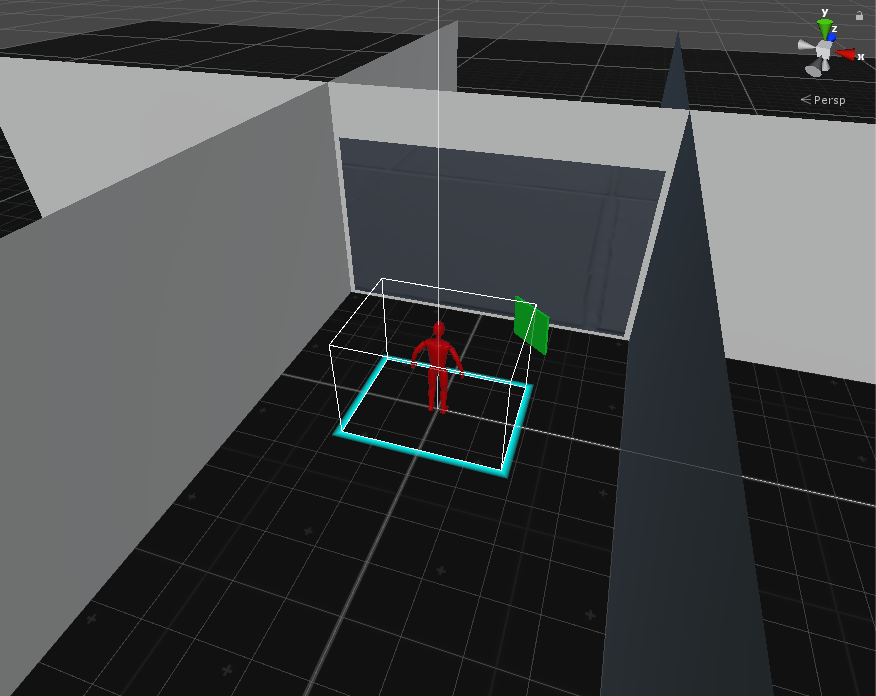
\includegraphics[width=\textwidth]{Bilder/Game/AltesSetup.png}
  }
  \caption[Altes Setup der Anwendung]{Ein sehr früher Prototyp der Anwendung in Unity}
  \label{fig:oldSetup}
\end{figure}

In Abbildung \ref{fig:oldSetup} ist ein früher Prototyp der Anwendung dargestellt. Erst später in der Entwicklungsphase wurde die rote farbe des Avatars in ein hellbraun umgeändert, da die Farbe zu sehr den Hazards glich.

\section{Hypothese}
Die Immersion des Systems mit den Trackern ist nach meiner Definition der Immersion messbar höher. Das liegt daran, dass die Tracker dem Benutzer mehr Kontrolle über den Avatar geben. Statt drei Kontrollierbaren Punkten im Aufbau ohne Tracker liefert der Aufbau mit Trackern neun Kontrollierbare Punkte und virtualisiert somit mehr Reize des Gehirns.
Aufgrund der erhöhten Immersion mit Trackern wird vermutet, dass das Embodiment durchschnittlich ebenfalls erhöht wird, da Embodiment eine Reaktion auf Immersion ist. Vor allem der Bereich Agency von Embodiment wird in dem Experiment angesprochen, daher sollte der größte messbare Unterschied zwischen den Gruppen in der Kategorie Agency sein.
Die Performanz sollte sich im Schnitt ebenfalls erhöhen, da die Tracker mehr Kontrolle der Beine erlauben und sich die meisten Objekte auf dem Boden befinden. Ein bekanntes Problem von VRIK mit drei Punkte tracing ist zusätzlich das verzögerte hinterher schweben des Körpers hinter dem Kopf, was Ausweichen schwieriger macht. Trotz der vermutlich unterschiedlichen Performanz wird die gefühlte erreichte Leistung der Probanden vermutlich in beiden Gruppen ähnlich sein, da die Gruppen nicht von der jeweils anderen Gruppe wissen.
Aus den genannten Annahmen ergeben sich folgende drei Hypothesen, welche untersucht werden sollen:
\begin{itemize} 
\item \textbf{H1 Embodiment:} Der Grad an Kontrolle über einen selbst-Avatar hat Auswirkungen auf das Embodiment.
\item \textbf{H1 Workload:} Der Grad an Kontrolle über einen selbst-Avatar hat Auswirkungen auf den gefühlten Grad an Belastung hinsichtlich der Aufgabe.
\item \textbf{H1 Punktzahl:} Der Grad an Kontrolle über einen selbst-Avatar hat Auswirkungen auf den Erfolg in einer Bewegungsorientierten Aufgabe.
\end{itemize}


\section{Hardware}
Bei dem Versuch kommt die HTC Vive als HMD zum Einsatz. Das Headset dient dem Avatar als Ankerpunkt für die Kamera in der Anwendung. Diese ist ein wenig unter den Augen des Avatars gelegen, da so die Animation durch IK besser funktionierte. Die Vive benötigt zwei höher gelegene Kameras, welche in dem Raum an einem Gerüst festgemacht sind. Mithilfe eines Tablets und der App \textit{Osram Lightify} können die Kameras aus der Entfernung ein und ausgeschaltet werden. Die Kameras sind für das Tracking im Raum zuständig und decken in meinem Fall ungefähr drei Meter mal fünf Meter ab. Dieses Gebiet wird in SteamVR kalibriert und dient im Spiel als begehbares Gebiet für den Spieler.
Dazu kommen zwei VIVE-Controller, deren Position ebenfalls von den Kameras erfasst werden. In jeder Hand wird ein Controller gehalten, daher steuert die Position der Controller die Position der Hände in der Anwendung.  Der Aufbau beider Versuchsgruppen ist bis zu diesem Punkt genau gleich.
Bei Versuchsgruppe zwei werden zusätzlich zu dem oben genannten sechs VIVE Tracker verwendet. Die Konfiguration, wo die sechs Tracker angebracht werden können, variiert stark. Theoretisch gesehen können die Tracker an jeglichem Objekt oder überall am Körper festgemacht werden. Das verwendete Avatarrig von VRIK besteht aus [[ca. 30]] verschiedenen Knochen ausgenommen der Finger und Zehenknochen. Standardmäßig vorgesehene Targets für Tracker gibt es in VRIK 10. Da die HMD und die Controller bereits drei davon abdecken, konnten die möglichen Tracking Ziele auf sieben begrentzt werden. Da alle konfigurationen, die einen Tracker an der Hüfte beinhaltetetn, Probleme verursachten, konnte die optimale konfiguration für sechs Tracker festgelegt werden. Die durch Gruppe zwei getrackten Körperteile sind also der Kopf durch die HMD, die Hände durch die Controller sowie jeweils beide Ellbogen, Knie und Füße mithilfe der Tracker. 
Die Tracker werden mithilfe von 1/4 Zoll Kamersastativschrauben an beidseitigen Klettbändern befestigt, welche leicht am Körper angebracht werden können. Da neben der Position auch die Rotation der Tracker relevant ist, wurden die Tracker in den Versuchen immer mit der Seite des Lichtpunkts nach unten gedreht.
Trotz der Tracker kommt bei Gruppe zwei IK zum Einsatz, da Knochen des Rigs wie die Hüfte, die Wirbelsäule oder die Schultern nicht getrackt werden und sich so natürlicher bewegt.

\section{Versuchsaufbau}
Der Proband befindet sich in einem quadratischen Raum ohne Decke. Die komplette Wand vor dem Spieler besteht aus einem virtuellen Spiegel. Die Fläche des Raumes ist ungefähr doppelt so groß als das begehbare Gebiet des Spielers. SteamVR zeigt automatisch ein rotes Netz dort an, wo das begehbare Gebiet aufhört, damit der Spieler nicht gegen Sachen außerhalb seiner freien Fläche stößt. Zusätzlich erstellte ich zusätzlich gelbe Indikatoren für das Gebiet auf dem Boden, da das Netz von SteamVR nicht in dem Spiegel angezeigt wird. Auf dem Spiegel befindet sich eine Punkteanzeige.
Abbildung \ref{fig:povSetup} zeigt die Sicht des Probanden zum Zeitpunkt des Starts der Anwendung. Unmittelbar vor dem Spieler befinden sich die beiden wichtigen Spielelemente und dienen als minimalistisches Tutorial. Rechts von dem Spieler befindet sich wenige Schritte entfernt eine grüne Fläche mit der Aufschrift \textit{Start}. Das Tutorial zeigt einen roten Quader, welcher die Objekte zum Ausweichen darstellt, in Nachfolgendem \textit{Hazards} genannt. Darauf ist eine \textit{-1} abgebildet, da dem Spieler für das Berühren eines roten Quaders ein Punkt abgezogen wird. Daneben befindet sich eine grüne Kugel mit der Aufschrift \textit{+2}, die die Objekte darstellt, die der Spieler während des Spiels einsammeln soll, um pro Stück zwei Punkte zu bekommen. Die grünen Kugeln werden im Nachfolgenden \textit{Collectibles} genannt. Das Ziel des Spiels sowie die einzelnen Elemente, die wichtig für den Spielablauf sind, werden dem Spieler bereits vor dem Aufsetzen des Head Mounted Displays (HMDs) erklärt und dienen hier nur zur zusätzlichen Verdeutlichung der Spielelemente. 
Das Startfeld muss berührt werden damit der Durchlauf des Spiels beginnt. Das Startfeld befindet sich zwei Schritte entfernt von der Startposition des Spielers in der Mitte des begehbaren Raums, damit das Spiel nicht unwillentlich durch eine falsche Geste gestartet wird und soll dem Spieler ein erstes Gefühl für die Einschätzung der Distanzen in der virtuellen Umgebung geben.

\begin{figure}[h]
  \makebox[\textwidth]{
    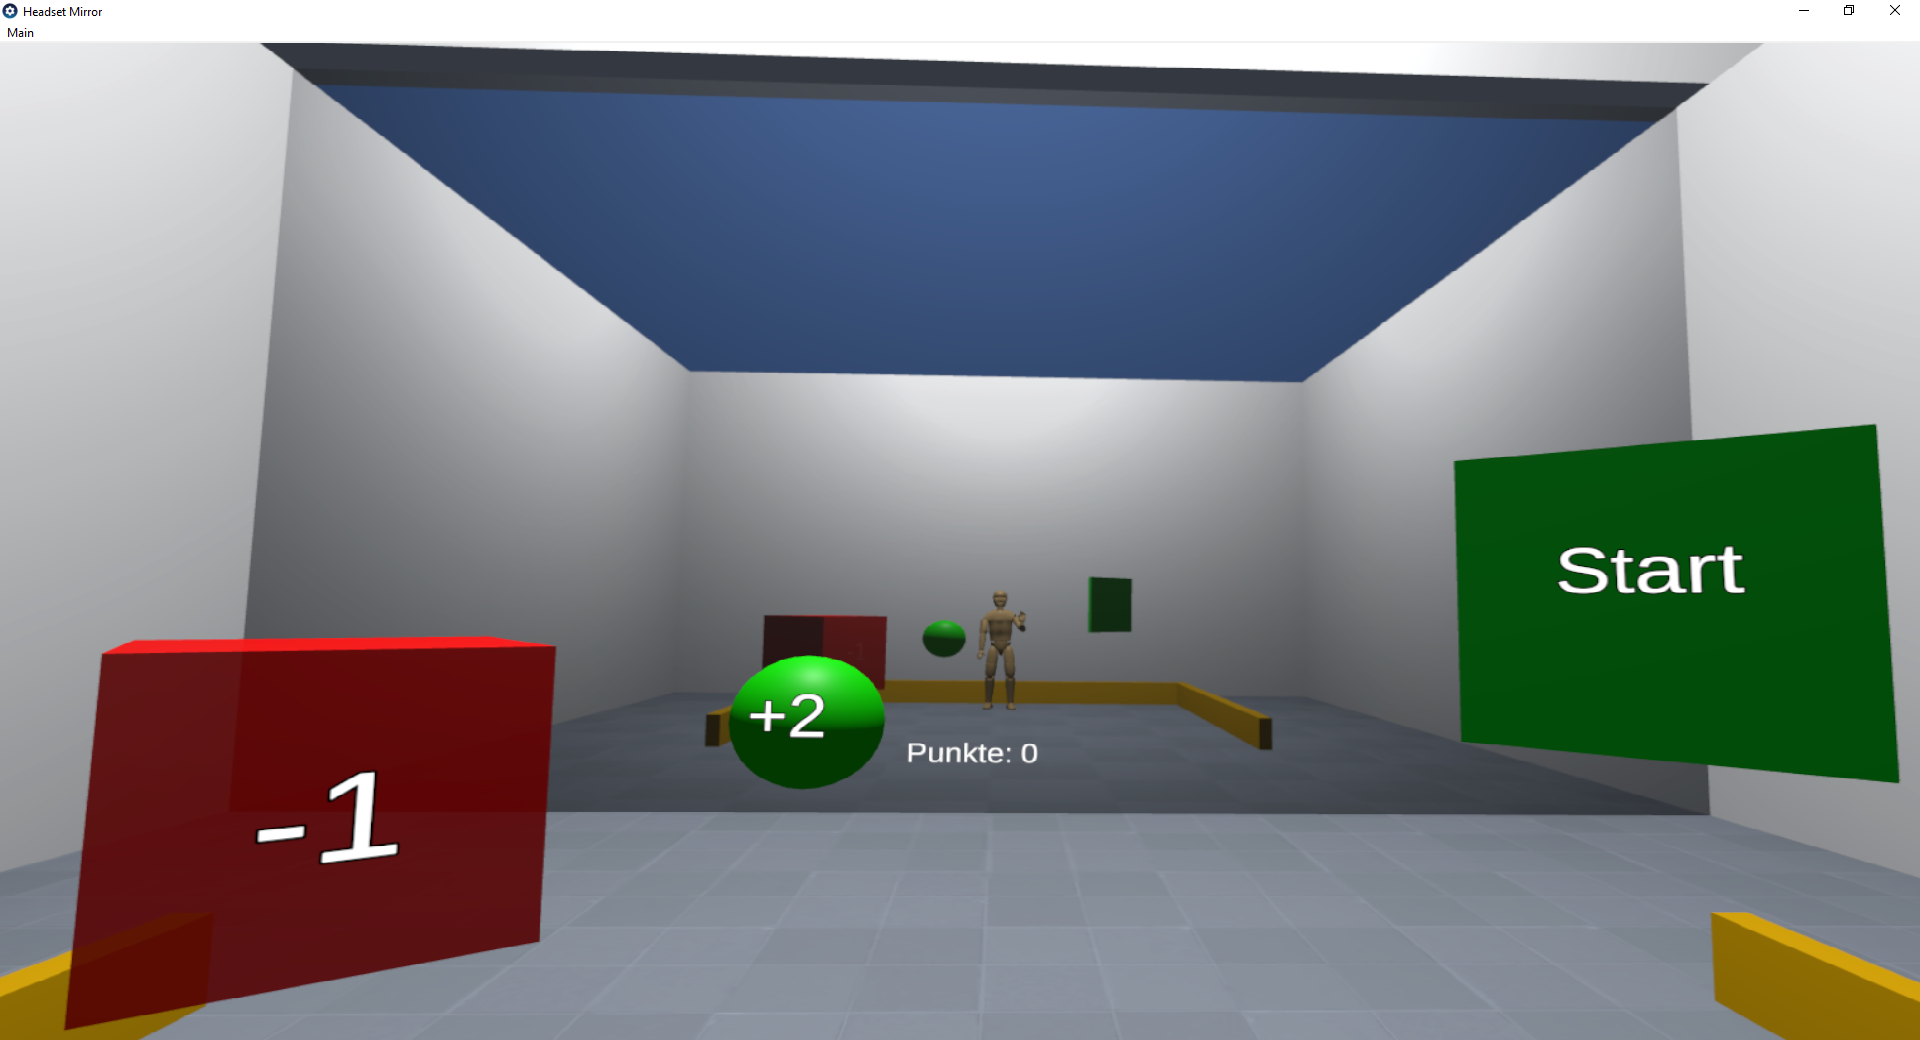
\includegraphics[width=\textwidth]{Bilder/Game/ingame.png}
  }
  \caption[Aktuelles Setup der Anwendung]{Sichtweise des Probanden wenn das Spiel gestartet wird.}
  \label{fig:povSetup}
\end{figure}

Die komplette Anwendung verzichtet auf Tasteneingaben des Benutzers, alle benötigten Eingaben passieren durch Berührung des Avatars mit den Objekten.
Sobald das Spiel gestartet wurde, bewegen sich von vorne aus dem Spiegel die Hazards und Collectibles in einem bestimmten Intervall und bewegen sich durch das begehbare Gebiet bis sie wieder aus der Rückwand verschwinden. Die Position der einzelnen Objekte wird vor dem Spiel zufällig innerhalb einem bestimmten Gebiet festgelegt. Zusätzlich können alle Objekte mit einer Wahrscheinlichkeit von 20 Prozent in der Luft schwebend statt auf dem Boden erscheinen. Dies soll den Spieler anregen, sich in gewissen Situationen zu ducken, um einem Hazard auszuweichen oder seine Hände zu bewegen um ein Collectible, welche über einem Hazard schwebt, einzusammeln. Während der gesamten Zeit wird dem Spieler seine Punktzahl angezeigt. Nachdem 40 Hazards und 20 Collectibles erschienen sind, ist das Spiel vorbei. Somit ist die höchste zu erreichende Punktzahl 40 und die niedrigste zu erreichende Punktzahl -40. Neben der gesamten Punktzahl werden bei Spielende die jeweils getroffenen Hazards und Collectibles angezeigt.
Sobald das Spiel beginnt, wird der Avatar ausgehend von der Position der HMD in alle Richtungen Skaliert. Das wirkt der unterschiedlichen Körpergröße bei verschiedenen Personen entgegen, da der Avatar bei kleineren Personen gebeugt steht oder bei größeren Personen den Boden nicht berührt.
mehr zum durchlauf



\section{Engine}
Die Anwendung wurde mithilfe der Unity Engine 2018.3.11f umgesetzt.
Unity bietet über den \textit{Assetstore} die Möglichkeit, Programme von Drittanbietern leicht in die eigene Anwendung zu integrieren. Die wichtigsten eingesetzten Assets für die Anwendung waren \textit{FinalIK} von rootmotion\cite{rootmotion} sowie SteamVR von Valve. FinalIK bietet vorgefertigte IK-Lösungen für eine Reihe an Anwendungsarten. Das im Experiment benutzte IK-Rig stammt von dem FinalIK Anwendungsbeispiel VRIK. Abbildung X zeigt die Standardkonfiguation der Knochen von VRIK. SteamVR bietet Grundfunktionalitäten für die HTC VIVE wie das Kamerarig und die Position der Controller. Die Textur für den Boden stammt ebenfalls aus SteamVR.


\section{Probleme}
Die größte Herausforderung während des Entwickeln als auch während des Versuchs war die große Anzahl an eingesetzter Hardware. Oft wurden scheinbar ohne Grund entweder die Tracker oder die Controller nicht erkannt oder konnten sich nicht mit SteamVR verbinden. Dies führte beim Versuch bei wenigen Testpersonen zu verminderter Immersion, da sie z.B. trotz Tracker ihren Ellbogen nicht bewegen konnten. 
Eine weitere Herausforderung war die Zuweisung der Tracker in Unity. Die SteamVR Anwendung besitzt kein benutzbares System, wie die Tracker konsistent dem gleichen Körperteil zugewiesen werden können. Letztendlich konnte ich im Code selbst die Zuweisung mithilfe der Herstellungsnummer der Tracker lösen.
Das Festmachen der Tracker am Körper bereitete ebenfalls viele Sorgen. Die Vive Tracker werden standardmäßig ohne Bänder zum Befestigen geliefert. Desweiteren gibt es keine offiziellen Bänder von Vive selbst. Meine Lösung beinhaltete beidseitiges Klettband mit Löchern für die von den Trackern benötigten Schrauben. Diese sind aber schwierig am Körper zu befestigen, wenn sie nicht rutschen sollen und sind anfällig dafür, dass die Tracker während der Anwendung rotieren.
 
